\graphicspath{{chapters/introduction/images/}}
\chapter{Introduction}

\label{sec:neutrinos}
\section{Neutrinos}
In 1896, Henri Becquerel discovered radioactivity in uranium \cite{Becquerel}.
Measurements over the following decades showed various types of nuclear decays based on the penetration depth of the ionizing emissions [rutherford?].
Measurements of one type of radioactivity, the beta decays, over the following 30 years showed that the production of two observed particles from one parent nucleus: a daughter nucleus and an outgoing electron.
A single body decay of this type produces a simple spectrum due to conservation of energy and momentum.
Indeed, the energy of the daughter nucleus and the electron are completely determined by these two conditions, leading to a narrow line emission spectrum.

Contrary to expectations, however, the measurement of energies of the two resulting particles showed wide, continuous spectra \cite{Chadwick}. 
The spectrum provided a major puzzle for physicists due to the contradition with the simple theoretical expectations.
A conundrum for many years, one possible solution was suggested in 1930 by Wolfgang Pauli.
In his letter, Pauli suggested that the conservation of energy and momentum could be saved if '... there could exist in the nuclei electrically neutral particles... which have spin 1/2 and obey the exclusion principle, and additionally different from light quanta in that they do not travel with the velocity of light' \cite{Pauli-Nu}.
The solution to the beta decay puzzle was, then, that this additional 'neutron' particle was emitted simultaneously with the observed daughter particles.
This newly proposed particle would be electrically neutral and, therefore, unable to be seen through traditional methods.
The resulting spectrum of the observed particles could then be continuous, as verified experimentally.

Pauli's suggestion provided a way to save the beloved conservation laws in physics, but at the expense of the assumption of a new particle.
The particle, called the 'neutron' in Pauli's letter and later renamed the 'neutrino' by Fermi, was proposed to be electrically neutral and, therefore, completely undetectable at the time.

It was not until nearly 20 years later, in 1956, that this mystery particle was first detected \cite{Cowan-Reines}. 
In a groundbreaking work, Cowen and Reines presented an experiment at the Savannah River Plant demonstrating detection of the neutrino.
The experiment, made up of layers of scintillation detectors around polyethelene boxes, yielded a signal-to-background rate of about 3 to 1 with a rate of 2.88 $\pm$ 0.22 counts/hour with a total livetime of 1371 hours, including time during which the nearby nuclear reator was offline.
For the discovery of the first neutrinos, Frederick Reines was granted a shared Nobel Prize in Physics for the year 1995 \cite{NobelPrize:1995-Reines}.

The experiment at the Savannah River Plant conclusively demonstrated the observation of neutrino events. 
Not long after, however, additional wrinkles in the story of the neutrinos emerged.
In 1962, an experiment performed at Brookhaven National Laboratory reported a new type of event: a neutrino candidate that produced only muons \cite{Danby-NuMu}, a new species of lepton discovered earlier that shared some properties with electrons, but with larger masses \cite{Neddermeyer-Muon}.
The neutrinos observed by Cowen and Reines interacted via inverse beta decay, producing the beta particle, now known to be an electron, in the process.
The observed neutrinos at Brookhaven, however, produced only muons.
These neutrinos appeared to produce no electrons in the interaction, indicating that a second kind of neutrino had been discovered.

For many years, the two neutrinos, dubbed the electron neutrino ($\nu_e$) and muon neutrino ($\nu_\mu$) due to their interactions with electrons and muons respectively, were studied in some detail. 
It wasn't until a series of experiments in the 1970s that significant information about the neutrinos again emerged.
Measurements at SLAC by Martin Perl and colleagues in 1974 and 1977 using a then-new $\mathtt{e^+ - e^-}$ collider showed anomolous events \cite{Perl-Tau}.
Conservation of energy and momentum once again appeared to be violated in reactions of the form 

\begin{equation}
	e^++e^- \rightarrow e^{\pm} + \mu^{\mp} + \mathtt{undetected particles}
\end{equation}

In order for the conservation laws to hold, two additional particles were required.
These particles would possess higher masses than the then-known electron and muon particles, but with an identical charge.
Perl suggested that the new particle, dubbed the tau lepton, could explain the result.

With the addition of a new charged lepton, theorists immediately predicted a third neutrino as well.
The new tau neutrino, $\nu_\tau$ remained solely a theoretical prediction until 2004, when the DONuT (\emph{D}irect \emph{O}bservation of \emph{N}u-\emph{T}au) collaboration published their first results.
In the initial paper, the DONuT experiment identified 4 candidate tau neutrino events with an estimated background of 0.34 events \cite{DONUT-2001}.
A total of 9 events were detected by the DONuT collaboration between 1997 and 2007, when the experiment ended \cite{DONUT-2007}.

Searches for additional neutrinos beyond the discovered three have been performed.
The cross section of the Z boson decaying to hadrons, for instance, is affected by the number of active, light neutrino species.
A precision measurement of the Z resonance completed at the LEP coillider demonstrated the existance of exactly three neutrinos \cite{ALEPH-3Nu}.

\begin{figure}
\centering
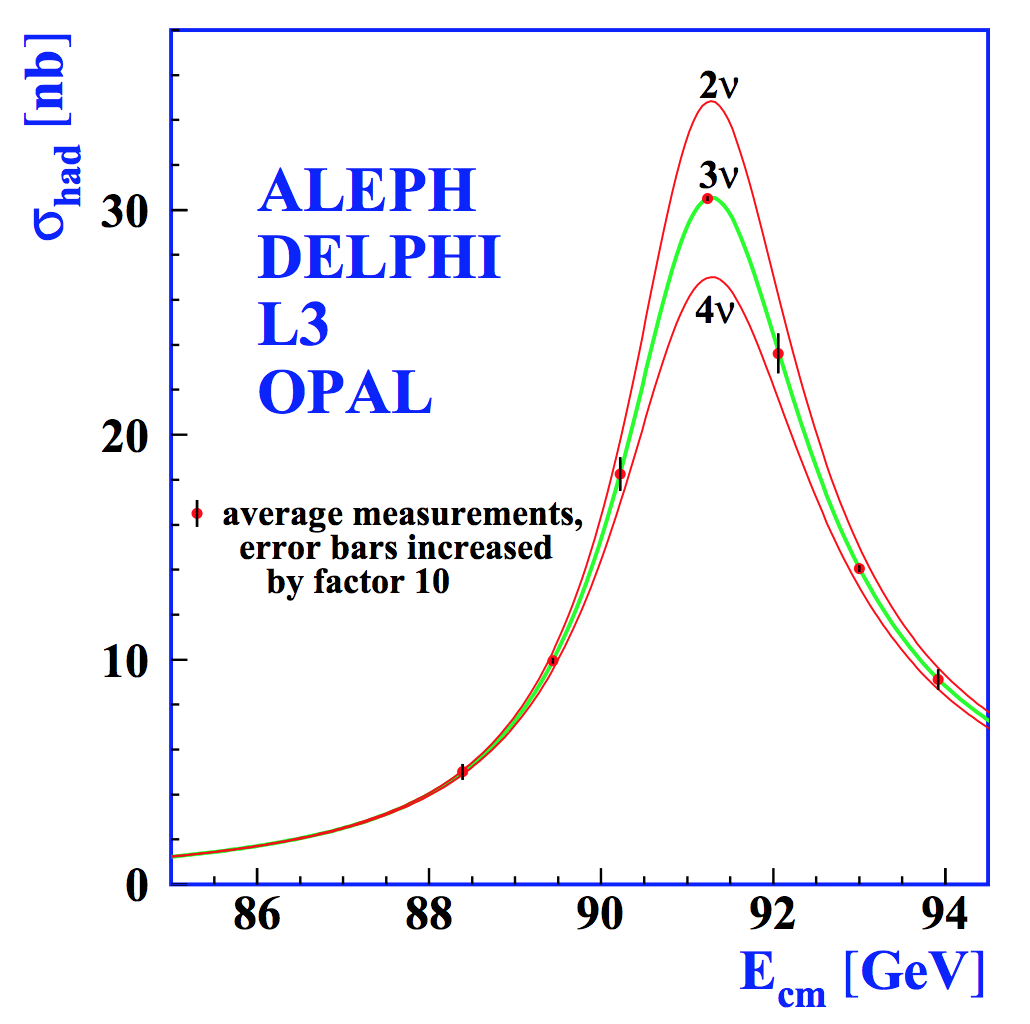
\includegraphics[width=0.5\linewidth]{ALEPH_NumNu.png} 
\label{fig:ALEPH}
\caption{The number of active neutrinos as measured by ALEPH, DELPHI, L3, and OPAL. The data from the four experiments strongly favors only three neutrinos coupling to the Z boson. Image taken from \cite{ALEPH-3Nu}.}
\end{figure}

\label{sec:cosmic_rays}
\section{Cosmic Rays}
In the early years of the 20th century, scientists began investigating previously-unknown ionizing radiation in the atmosphere.
Scientists using electroscopes, early instruments designed to measure electric charge and radiation, discovered low levels of radiation in the air.
This new radiation was observed to be reduced when the electroscope was shielded by metal free of radioactivity, indicating that the signal was not an artifact of the detector itself and was, instead, coming from an external source.

Following just a few decades after the discovery of radioactivity by Becquerel, many scientists believed that the electroscope was picking up radiation from the Earth itself.
The rate would be expected to decrease with increasing altitude above sea level and, to increase with increasing depth in the sea.
Early measurements by Domenico Pacini in 1910 showed that the radiation rate decreased by 20\% at a depth of 3 meters underwater compared to the rate at the surface \cite{Pacini-CRSource}, implying an origin independent of the Earth's crust.
Measurements were performed with electroscopes by Victor Franz Hess in 1912 tested the rate of ionizing radiation up to an altitude of 5 km \cite{Hoerandel-CRHistory}.
Hess showed that the observed rate decreased until an altitude of around 1 km, but at a slower rate than expected from theory.
Above 1400 meters, however, the rate of ionizing radiation increased again, rising substantially up to the maximum altitude reached at 5300 meters \cite{Compton-CRAltitude}.
Hess's work, later confirmed by Henri Millikin, showed definitively that there exists a source of radiation of extraterrestrial origin, earning him the Nobel Prize in Physics for 1936 \cite{NobelPrize:1936-Hess}.
This radiation was later dubbed "cosmic rays" by Millikan in reference to their extraterrestrial origin.

Work on cosmic rays has lead to numerous discoveries.
In 1937, for example, scientists working at an altitude of 2300 meters above sea level using photographic plates to study cosmic rays discovered interactions labeled "stars" \cite{Blau-HadronicShowers}. 
These "stars" showed multiple outgoing particles from a single vertex.
Further work on these types of events lead to the discovery of hadronic interactions, paving the way for the use of photographic emulsions in the study of particle physics.

In 1929, Bothe and Kolhoerster introduced the coincidence technique in which two or more detectors could be read out only when all participating detectors detect signals \cite{Kolhoerster-CoincidenceDetectors}.
The dawn of coicidence counters led to the remarkable observation that cosmic rays had a considerably larger extent than expected.
While the original objective was to determine the random coincidence rate between two counters, the coupled Geiger-Mueller counters showed coupled behavior out to a distance of at least 75 meters.
Work by Pierre Auger later confirmed the findings of Kolhoerster \findref{P. Auger et al., Comptes renduz 206, 1721 (1938)}.

\begin{figure}[!h]
\centering
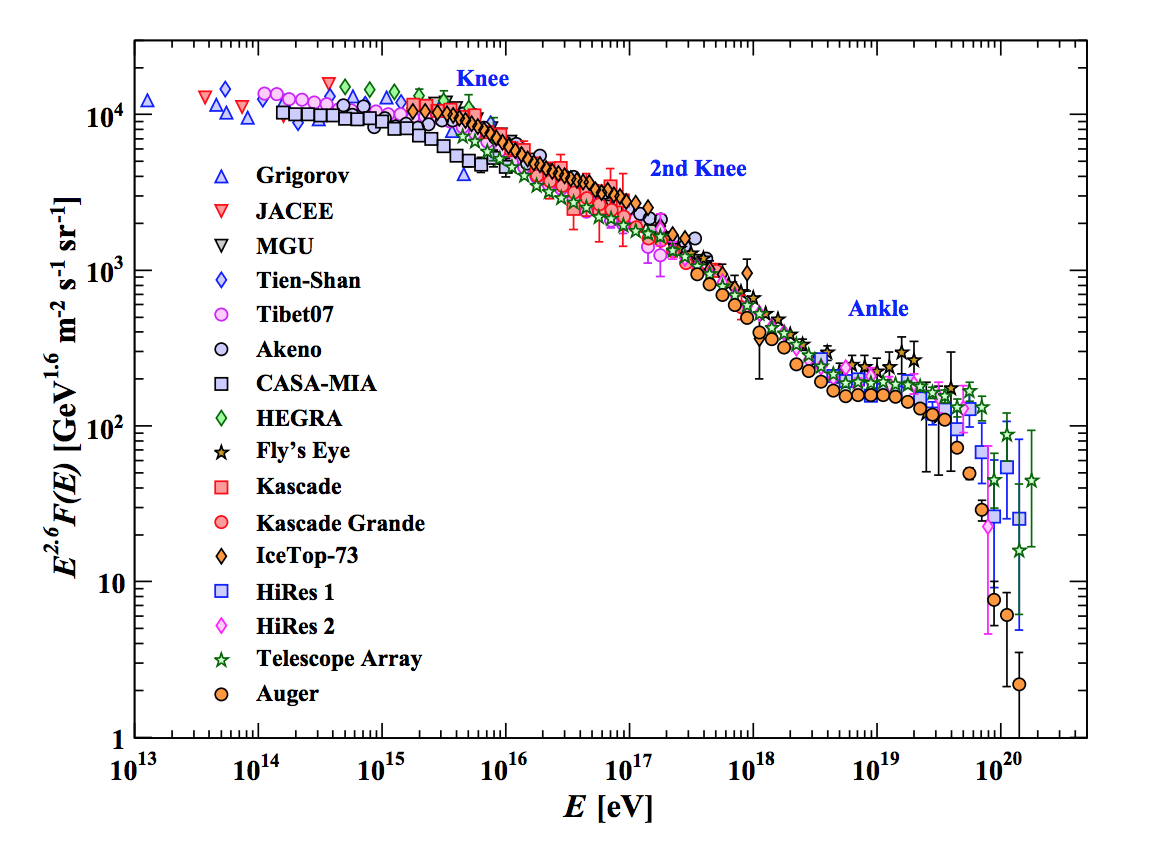
\includegraphics[width=0.9\linewidth]{CR_Spectrum_PDG15.png}
\label{fig:CR_spectrum}
\caption{The cosmic ray spectrum covers many orders of magnitude and has been verified by many experiments to high precision. The various features are thought to be caused by multiple sources at different scales. Image taken from \cite{PDG-2015}}
\end{figure}

Instead of consisting of single particles reaching detectors, Kolhoerster showed that the detected particles were due to extended air showers originating from cosmic ray interactions high in the atmosphere.
These showers begin with a cosmic ray primary particle, often a single proton accelerated to high energies, which interacts with particles of the Earth's atmosphere.
The interaction leads to the creation of various daughters, including neutrinos, muons, pions, kaons, and other hadrons.

Modern measurements have shown that the cosmic ray spectrum primarily consists of protons with a small contribution from helium and heavier elements \cite{PDG-2015}
These ions are accelerated in unknown astrophysical sources up to extremely high energies.
The cosmic ray spectrum extends over many orders of magnitude, with the highest energy observations reaching $\mathtt{10^{20}}$ electronvolts - far higher than any Earth-based accelerator.
The spectrum has multiple features that are believed to arise from different accelerator sources at different scales.

\label{sec:standard_model}
\section{The Standard Model}

\begin{figure}
\centering
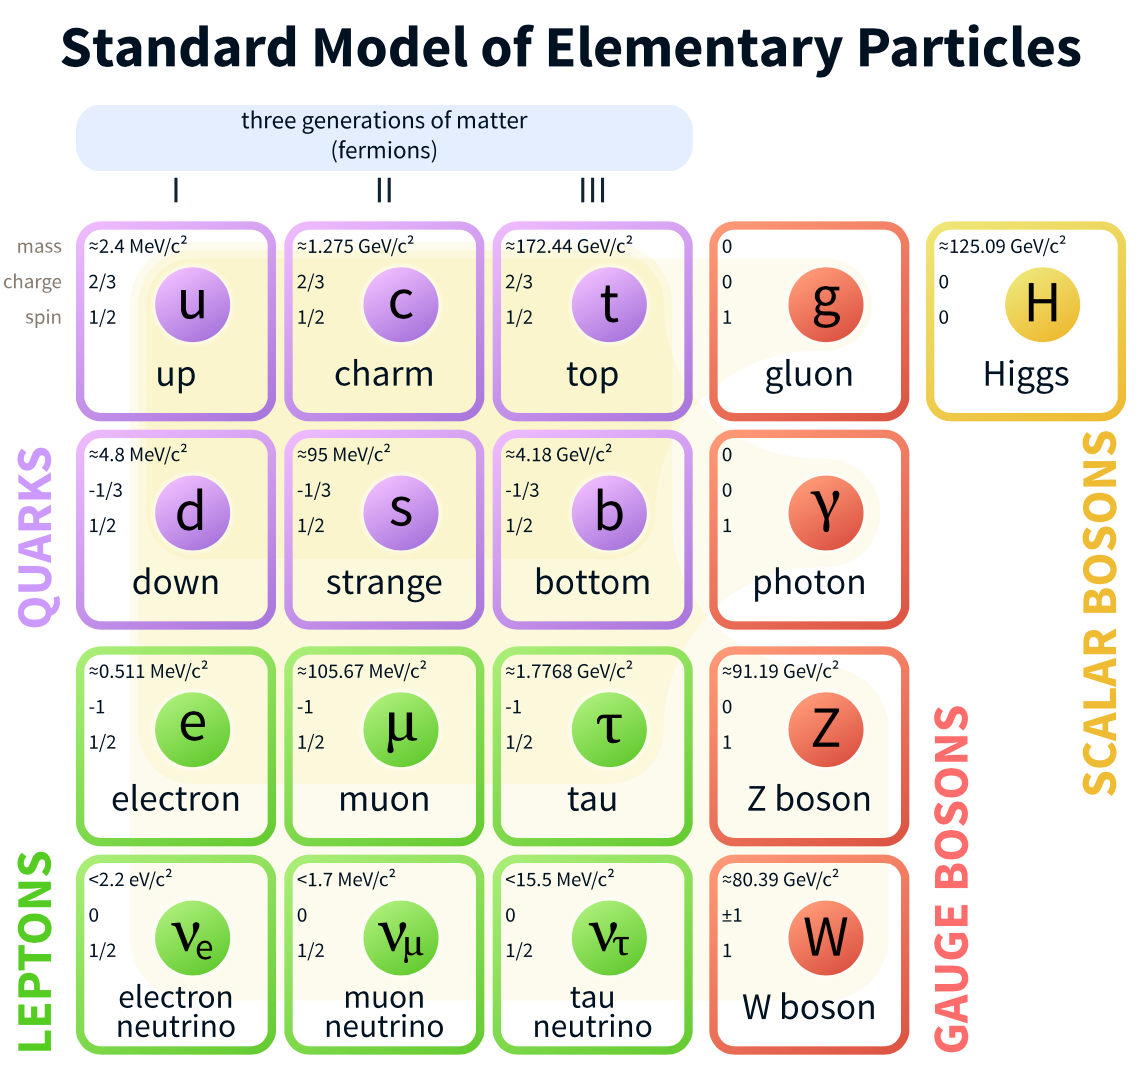
\includegraphics[width=0.7\linewidth]{Standard_Model_of_Elementary_Particles.png}
\label{fig:standard_model}
\caption{The Standard Model of particle physics is made up of charged and uncharged leptons, quarks, and the various bosons. Image taken from \cite{StandardModel-Image}}
\end{figure}

These particles form just a small part of the Standard Model of particle physics.
The Standard Model consists of six quarks (up, down, strange, charm bottom, and top), three charged leptons (electron, muon, tau), three uncharged leptons (electron neutrino, muon neutrino, and tau neutrino), and the five bosons related to interactions (photon, Z, W, gluon, and Higgs).
Combinations of the quarks lead to various hadrons, paticles which interact with and are formed via the strong force, with different combinations of quarks and anti-quarks producing a wide variety of particles.
The Standard Model, developed over the last half century, elegantly encapulates the range of phenomena known to occur in particle physics and has been verified repeatedly over decades by many experiments.
Predictions of the Standard Model have been carefully verified by accelerator experiments, yielding precise checks on a wide range of parameters.

The three charged leptons and neutrinos form three 'families' or 'flavors'. 
Each charged lepton posseses a coupled neutrino which shares a lepton number conserved in interactions.
The electron, the lightest of the charged leptons at 511 KeV \cite{PDG-2015}, is a key ingredient of the atoms that make up the world, forming the basis for all of chemistry and is the only stable charged lepton.
The muon, with a mass of 105.7 MeV, is the middle of the three charged leptons, often appearing in particle interactions accompanied by the muon neutrino.
The muon has a relatively long livetime of 2.197 microseconds, far longer than many unstable hadrons.
The tau lepton is the heavies of the leptons, and with a mass of 1.777 GeV, it is heavier than the proton and appears only in relatively high energy interactions.
The tau has an extremely short lifetime, at 290.6 femtoseconds, and a rich variety of decay products.
This extremely short lifetime and high mass make the tau difficult to produce and study.

For the purposes of this work, the most significant parts of the Standard model are the neutrinos, which will be defined to be signal events; the up and down quarks, which will make up the protons and neutrinos upon which the neutrinos will interact; the W and Z bosons, which mediate the weak interactions via which the neutrinos may be observed; and the photon, which gives a method of observation of the interactions.

\label{subsec:interactions}
\subsection{Neutrino Interactions}
In the Standard Model, neutrinos are assumed to be massless, left-handed spin-1/2 leptons which interact solely via the weak force.
Neutrinos, therefore, are only visible via indirect effects, such as scattering or production of charged particles that may, in turn, give off their own visible signature.
An understanding of the methods by which neutrinos are detected therefore forms an important basis for the study of these elusive particles.
Two basic Feynman diagrams, shown in Figure~\ref{fig:nu_vertex}, may be used to represent the interaction verticies.

\begin{figure}
\centering
\begin{tabular}{@{}ll@{}}
\feynmandiagram [vertical=w1 to w2] {
  nue1 -- [fermion, edge label=\(\nu\)] w1 -- [fermion, edge label=\(l\)] e1 ,
  w1 -- [boson, edge label = \(W^{+}\)] w2
}; 
 & \feynmandiagram [vertical=w1 to w2] {
  nue1 -- [fermion, edge label=\(\nu\)] w1 -- [fermion, edge label=\(\nu\)] nu2 ,
  w1 -- [boson, edge label = \(Z^{+}\)] w2
}; \\ 
\end{tabular}
\label{fig:nu_vertex}
\caption{Feynman diagrams showing the interaction vertex of the neutrino with the W and Z boson.}
\end{figure}

From these two vertices, the various interactions relevent for this work may be derived.
During so-called \emph{charged-current} (\emph{CC}) interactions, a $\mathtt{W^{\pm}}$ boson is exchanged between a neutrino and target particle, in the process converting the uncharged neutrino to the corresponding charged lepton.
The \emph{neutral-current} (\emph{NC}) interactions are those in which the uncharged Z boson is exchanged with the target and the neutrino, although losing a fraction of the initial energy, does not get converted to a charged lepton.
Outgoing charged leptons in charged-current interactions may be detected, although the direction will not necessarily correspond to that of the incident neutrino. 
The average angle between the incident neutrino and outgoing lepton may be approximated following Equation~\ref{eqn:kinematic_angle}.

\begin{equation}
\bar{\theta_{\nu l}} \approx \frac{\mathtt{1.5^o}}{\sqrt{E_\nu \left[TeV\right]}}
\label{eqn:kinematic_angle}
\end{equation}

There exist three further classifications of neutral-current and charged-current neutrino interactions in the energy range used in this work: the quasi-elastic, resonant, and deep inelastic interactions \cite{Formaggio-Xsec}.
Each occurs at different energies, as shown in Figure~\ref{fig:xsec}.

\begin{figure}
\centering
\begin{tabular}{@{}ll@{}}
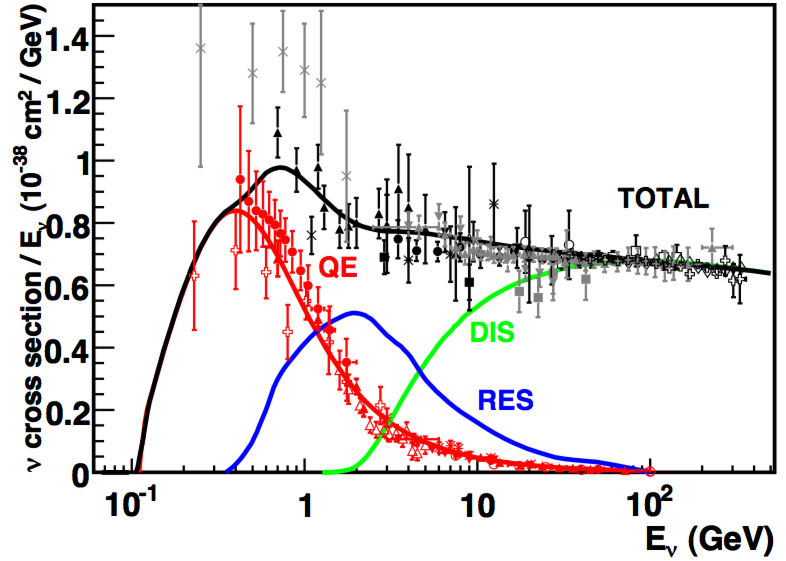
\includegraphics[width=0.4\linewidth]{nu_xsec_formaggio.png}
 & 
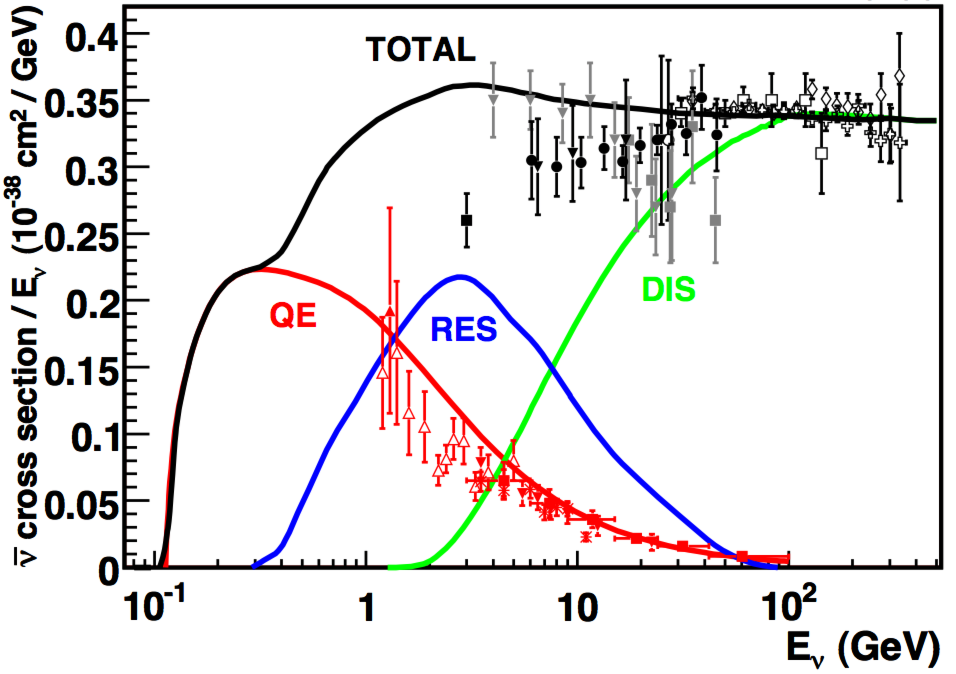
\includegraphics[width=0.4\linewidth]{nubar_xsec_formaggio.png}
 \\ 
\end{tabular}
\label{fig:xsec}
\caption{The relative contributions to the cross section for $\nu$ (left) and $\bar{\nu}$ (right). The QE events dominate below 1 GeV while the DIS events dominate above 10 GeV. Note the different scales for the neutrino and antineutrinos. Images taken from \cite{Formaggio-Xsec}}
\end{figure}

\subsubsection{Quasi-Elastic and Resonant Interactions}
At low energies of approximately 100 MeV to around 2 GeV, the neutrinos interact via \emph{quasi-elastic scattering} (\emph{QE}) interactions.
In the QE interaction, the neutrino scatters off an entire nucleon instead of the individual quarks.
In a charged current QE neutrino (anti-neutrino) interaction, the target neutron (proton) is converted to a proton (neutron) while the neutrino is converted to a charged lepton.

The cross section for QE interactions depends on various nuclear form factors that must be fit to experimental data.
Many of these form factors may be fit to electron scattering data, leaving only the axial vector nuclear form factors to be measured in the neutrino sector \cite{Formaggio-Xsec}.
This form factor is normally assumed to have the dipole form 

\begin{equation}
F_A\left(Q^2\right) = \frac{g_A}{\left(1+\frac{Q^2}{M_A^2}\right)^2}
\label{eq:axial_mass_eq}
\end{equation}

where $\mathtt{g_A}$ is a constant fit to experimental data, $\mathtt{Q^2}$ is the 4-momentum transferred in the interaction, and $\mathtt{M_A}$ is known as the "axial mass".
This last term is fit to experimental data with a value of $\mathtt{M_A = 0.999 \pm 0.011}$ GeV \findref{formaggio}.

\emph{Resonant scattering} interactions (\emph{RES}), which result in the excitation of a nucleon followed by decay via emission of (typically) pions, occur for neutrinos of slightly higher energies of around 500 MeV to 10 GeV.
Resonant interactions are modeled in a similar way as the quasi-elastic interactions, with an associated axial mass term used to describe nuclear uncertainties.

\subsubsection{Deep Inelastic Interactions}
Above a few GeV, the neutrino cross section rises approximatley linearly and is dominated by \emph{deep inelastic scattering} (\emph{DIS}) interactions.
In DIS events, the exchange of the Z or W boson probes the internal structure of the nucleons.
This results in disruption of the nucleon and the larger nucleus.
The collection of daughter particles form what is known as a \emph{hadronic shower}.


\label{sec:detection_methods}
\section{Methods of Detection}
Neutrinos may be detected through these various interaction channels, with each possessing a distinct signature.
For many events, the interaction of the neutrino leads to the emission of various hadrons in a hadronic shower.
This may be composed of many particles, as is the case with most DIS events, or it may consist solely of a limited number of pions, as is typical for RES events.

In addition to the hadronic shower, charged-current interactions possess an outgoing charged lepton, the result of which depends on the flavor of the lepton.
Outgoing electrons will often quickly scatter in interactions with the surrounding media, ionizing atoms and producing a secondary \emph{electromagnetic shower} of particles.
Muons, on the other hand, travel longer distances before scattering or being absorped in the medium, leading to an extended track.

The signature of a tau decay varies significantly.
Because the tau lepton has a very short lifetime, outgoing taus tend to decay immediately, producing daughter particles in a secondary hadronic shower that may or may not be spatially separated from the initial shower.

In each case, the charged particles deposit energy into the interaction medium during travel through a series of stochastic and continuous emissions.

\subsection{Stochastic Emission Mechanisms}
\begin{figure}
\centering
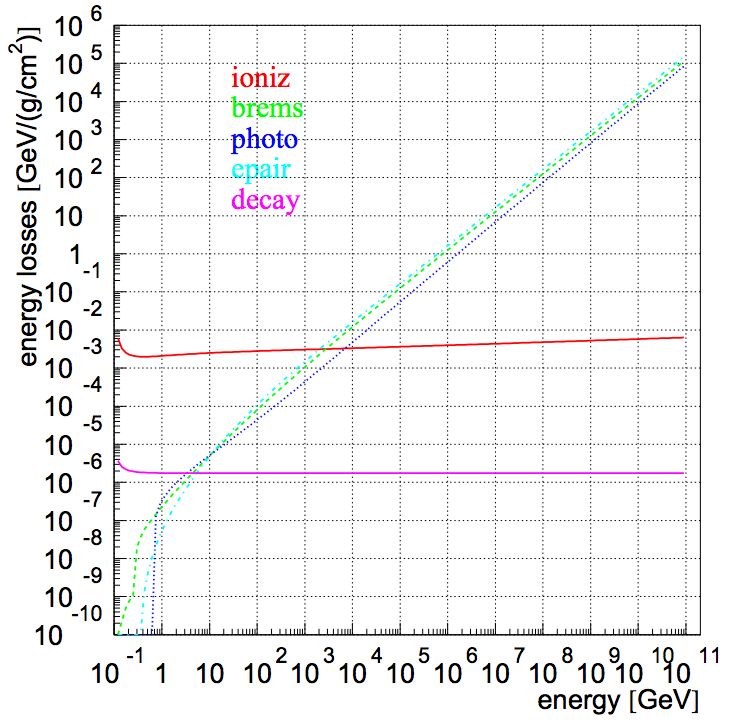
\includegraphics[width=0.6\linewidth]{discrete_emissions_MMC.png}
\label{fig:discrete_emissions}
\caption{Average energy losses ($\mathtt{\frac{-dE}{dX}}$) for a muon in ice. At very low energies, ionization losses dominate. Above approximately 1 TeV, pair production and photonuclear effects become more important. Image taken from \cite{Dima-MMC}}
\end{figure}
A total of five major stochastic emission mechanisms are important for the energy losses in neutrino experiments \cite{Dima-MMC}.
The simplest such mechanism is the decay of the particle, a process which splits the energy of the parent into multiple, lower energy daughters.
Decays can often by important in the identification of the neutrino type, particularly for tau neutrino candidates, which show a unique, background-free decay signature.

Ionization losses occur when the charged lepton interacts with electrons in the medium, transferring enough energy to librerate the electrons from bound states.
At low energies, these losses may be the most significant form of energy loss for charged particles, providing a significant source of additional electrons for detection.
Ionization losses occur roughly independently of the energy of the charged lepton.

For higher energies, radiative losses become important \cite{PDG-2015}.
Bremmstrahlung, photon emission from charged particles accelerating in a magnetic field, becomes one of the dominant sources of emission around 1 TeV.
Pair production, in which a particle and antiparticle (typically electron and positron) are created, is equally important.
At the highest energies, hadronic interactions of photons lead to still-stronger emission.

There exists a minimum in the energy loss rates.
Particles emitting near this minimum rate are known as \emph{minimum-ionizing} particles \cite{PDG-2015}.

\begin{figure}
\centering
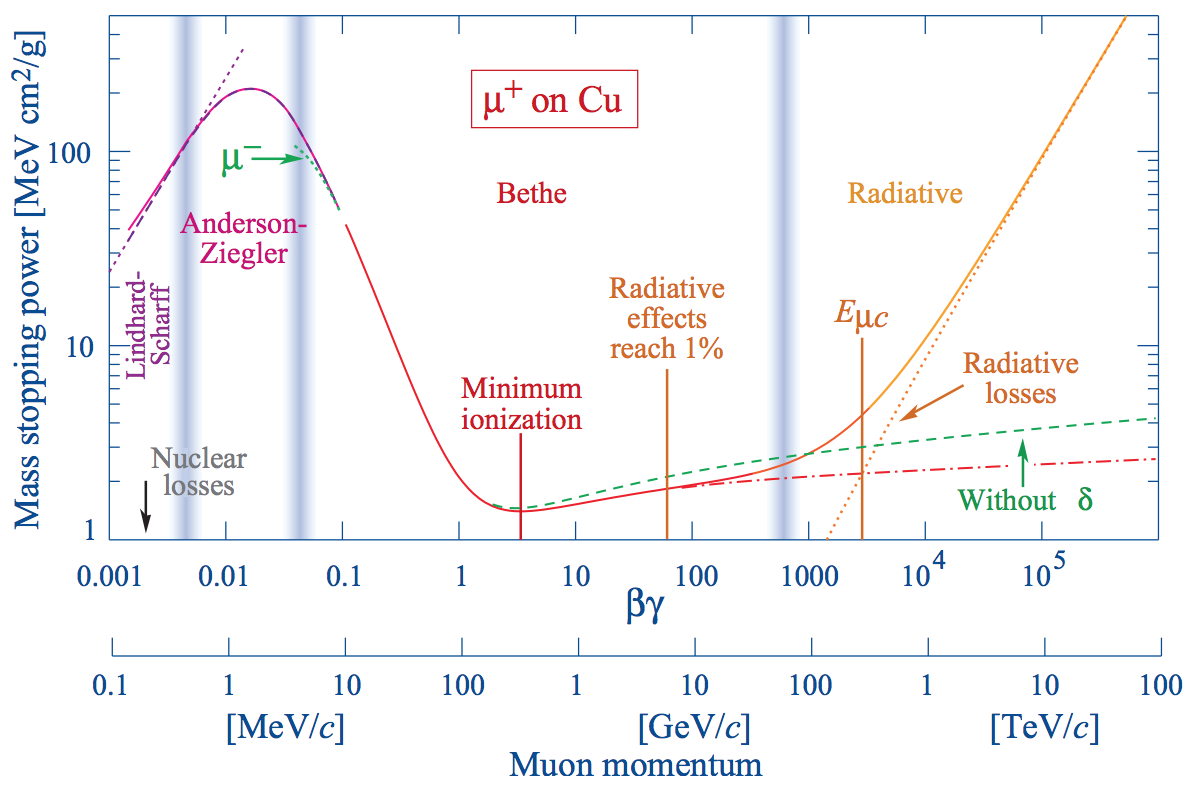
\includegraphics[width=0.8\linewidth]{bethe_bloche-PDG15.png}
\label{fig:discrete_emissions}
\caption{An example of the energy emission ($\mathtt{\frac{-dE}{dX}}$) calculated for muons incident on copper. Note the radiative losses due to bremsstrahlung, pair production, and photonuclear interactions at high energies. Note also the labeled minimum demonstrating the energy of a minimum ionizing particle. Image taken from \cite{PDG-2015}.}
\end{figure}

Stochastic emissions result in additional particles in the detector, leading to improved light yield.
In addition, some detectors use photosensitive emulsions  \cite{Description-OPERA, DONUT-2001}, scintillators \cite{Description-MINOS, Description-NOvA, Description-MINERvA, Description-T2K}, or time projection chambers \cite{Description-ICARUS2} in order to track ionization losses.
These emulsions yield precise characterization of particle decays, allowing experimentalists to uniquely determine the flavor state of the interacting neutrino.

\subsection{Cherenkov Emission}
When a charged particle passes through a dielectric medium with a speed larger than the local phase velocity of light, it will emit \emph{Cherenkov radiation}\cite{Cherenkov-Radiation-Confirmation}.
The effect, first reported by Pavel Cherenkov in 1934 \cite{Cherenkov-Radiation-Observation} remained unexplained theortically until work done by Ilya Frank and Igor Tamm in 1937 \cite{Frank-Tamm}.

For a dielectric medium, the electric field of the charged particle will polarize atoms in the medium by inducing a small dipole moment due to electromagetic effects in nuclei of atoms in the medium \cite{Griffiths-EM}.
The resulting disturbance of the medium propagates with the phase velocity of light in the medium, given by the speed of light, \textit{c}, and the index of refraction as a function of the frequency of light, \textit{n(\omega)}.
If the charged particle is traveling faster than the local phase velocity, the electromagnetic disturbance propagates with constructive interference, resulting in a planar wavefront of emission known as \emph{Cherenkov emission}.
The angle of the wavefront relative to the propagation direction is given by ratio of the distance traveled by the particle and photons in a given time.

\begin{equation}
cos(\theta_C) = \frac{\frac{c}{n(\omega)} t}{v t} = \frac{c}{n(\omega) v}
\end{equation} 

The energy threshold for Cherenkov emission is set by a combination of the particle mass and the local phase velocity for light, $\frac{c}{n}$.
Using the relativitistic kinetic energy \cite{Tavernier-Particles},

\begin{equation}
E_{C} \geq \frac{mc^2}{\sqrt{1-\left(\frac{c/n}{c}\right)^2}}
\end{equation}

\begin{equation}
E_{C} \geq mc^2\sqrt{\frac{n^2}{n^2-1}}
\end{equation}

For ice with a index of fraction of 1.32 at 400 nanometers \cite{ChinesePhysC-2014}, this works out to a minimum energy of 270 keV for electrons and 56.2 MeV for muons.
The number of photons emitted increases with energy, with approximately 50\% more photos produced in blue visible light than in red\cite{Tavernier-Particles}
The full emission spectrum, first worked out by Ilya Frank and Igor Tamm in 1937 \cite{Frank-Tamm}, depends on a number of parameters, including the energy and charge of the emitting particle as well as the properties of the medium.
In the case of a particle traveling a distance $L$ much larger than the photon frequency of interest, $\lambda$, the number of emitted photons may be approximated by

\begin{equation}
\frac{dN}{d\lambda}=\frac{2\pi \alpha}{\lambda^2}Lsin^2\theta_C \;\;\; L >> \lambda
\end{equation}

Cherenkov emission is not limited to a single charged lepton. 
All charged particles emit Cherenkov radiation, including any hadrons and charged daughter particles, resulting in measurable signals.
While the total amount of energy lost via Cherenkov emission is small relative to losses due to stochastic processes, this emission type is both continous and results directly in photons which may be observed by photodetectors.
This technique is used by multiple experiments, including SNO \cite{Description-SNO}, Super-Kamiokande \cite{Description-SuperK}, ANTARES \cite{Description-ANTARES}, and IceCube \cite{Description-IceCube}.

